 \chapter{Application of Machine Learning on Medical Data}
  \label{chpt:machine-learning}
 \nomenclature[1]{ANN}{Artificial Neural Network} 
 \nomenclature[1]{CNN}{Convoluted Neural Network}
 \nomenclature[1]{LSTM}{Long Short Term Memory}
 \nomenclature[1]{MLP}{Multi-Layer Perceptron}
  \nomenclature[1]{TF-IDF}{Term Frequency Inverse Document Frequency}
 \nomenclature[1]{NLTK}{Natural Language Toolkit}
 \nomenclature[1]{PPV}{Positive Predictive Value} 
 \nomenclature[1]{NPV}{Negative Predictive Value}
  \nomenclature[1]{TPR}{True Positive Rate}
  \nomenclature[1]{SVM}{Support Vector Machine}
  \nomenclature[1]{CART}{Classification and regression tree}
   \nomenclature[1]{KNN}{K-Nearest Neighbour}
    \nomenclature[1]{RF}{Random Forest}  
    
\section{Introduction}
 
 
%Outline the different factors that co-vary and the fact that there are many of them (from patient information to text etc. ) with complex interactions. 
%Explain how these interactions are too complex for  humans to decipher OR that they can do it but are too slow at doing it (too much data). 
%Essentially the motivation for using machine learning
%Then state what models are the most appropriate based on the type of data you have or the type of complexity within it (modelling complex sequences for instance etc.)
%Then briefly explain the structure of the models in the context of your data. 




Machine learning has been utilised in many industrial applications. Increased adoption of data mining and machine learning in competitive industry largely stems from the increased efficiency offered by knowledge extraction. Although not fully understood, humans tend to be strong at intuition, particularly when individuals can draw on past experiences to identify patterns \cite{okoli2016information,lyneham2008explicating}. In the context of this thesis we can assume human understanding relates to individuals with strong domain knowledge and local experience. Humans, in the medical domain, are generally seen as the gold standard in terms of diagnostics \cite{wang2018trusting}. However, humans are not as strong as computers in terms of their capacity to comprehend very large volumes of data, nor in their capacity to discern obscure connections between data. 
 
 A further consideration is that the multitasking capacity of machines far outpaces that of biological minds  \cite{singh2013designing,cherif2018multitasking} . This is relevant in a context where the domain experts discussed in this thesis are already fully engaged in roles relating to triage, treatment, and transcription. Analysing patterns from large quantities of data, in either a passive or active capacity, is neither demanded of nor a realistic competency of these staff.  
 
Nevertheless, even if the data presented proves ill-suited to human processing to provide predictions, that does not necessarily mean that a particularly complicated solution is needed to predict frequent user cases. This chapter will consequently discuss the information that relates to frequent users, and the ability of heuristics to accurately predict cases as belonging to frequent users based upon either parametric case details or case free-text\index{free-text} terms (that is to say, non-contextual lexical tokens). 

In Chapter \ref{chpt:background} we saw the types of parameterised data available in the corpus, including a description of FTN, such as the lexical diversity, number of words, and number of unique words in the notes, along with the number of free-text records in general. 

In order to establish a baseline in this research, traditional machine learning models\footnote{The author acknowledges that, conceptually, Neural Networks are as old as many of the other methods described in this chapter, but uses the term `traditional' relative to very recent developments in this particular field.} will be trained on the different types of data available in the corpus, with the results described below. 

First, the parametric data will be processed to make it suitable for machine learning algorithms. A variety of different methodologies will be employed in relation to this data to discover the entropy of the various data contained within parametric fields. Following this, simple approaches relating to the free-text data will be explored in terms of their capacity to predict frequent users. 

After assessing the performance of various machine learning techniques in relation to the data described above, the potential use of artificial neural networks (ANNs\index{Artificial Neural Networks}) will be introduced. The rationale for the use of ANNs\index{Artificial Neural Networks} will be made along with the approach for testing and developing a successful model. 

Finally, the viability of different approaches to potentially improve the quality of the data available within the corpus will be examined. Subsequent chapters will discuss the means that were ultimately adopted to this end, including the consequent  impact that this has upon predictive performance. 



 

 


 \section{Data Analysis}


\subsection{Metrics}
\label{section-metrics}

Training for the algorithms described in the rest of this chapter will use a downsampled training set relating to 50\% of frequent user cases, with testing scores reported below. Testing uses an imbalanced dataset of unseen cases. Because of the imbalanced nature of the dataset, a simple measure of accuracy provides a poor measure of the effectiveness of the predictive model. As such, when reporting testing accuracies in this chapter, we also detail the positive predictive values (PPV), often referred to as precision, and the negative predictive values (NPV). 

Other values reported during testing in this thesis include true positive rate (TPR) often referred to as recall, and the F1 measure (the harmonic mean of precision and sensitivity). These measures are defined as follows:


\begin{equation}
PPV = \frac{\text{True Positives}}{\text{True Positives + False Positives} }
\end{equation}

\begin{equation}
NPV = \frac{\text{True Negatives}}{\text{True Negatives + False Negatives} }
\end{equation}

\begin{equation}
TPR = \frac{\text{True Positives}}{\text{True Positives + False Negatives} }
\end{equation}

\begin{equation}
F1 = {\LARGE 2}\frac{\text{PPV * TPR}}{\text{PPV + TPR} }
\end{equation}

Data shown are means and standard deviations, unless otherwise noted.

 \section*{Approaches}

In the testing of parameterised and free-text data, the  following, well known algorithms were applied. 


\subsubsection{Naive Bayes\index{Naïve Bayes}}

The Naïve Bayes\index{Naïve Bayes} predictive model returns a  maximum \textit{a posteriori} estimate probability where the posterior probabilities for the levels of the target feature are computed under the assumption of conditional independence \cite{kelleher2015fundamentals}. This model has generally achieved good results in high dimensional contexts, notwithstanding its omission of the consideration of correlation between inputs. Optimal Bayseian classification is given as follows:


\[ \arg \max_{v_{j} \in V} \sum_{h_{i} \in H} P(v_{j}|h_{i}) P(h_{i}|D)\]

where \textit{H} is a set of candidate hypotheses for observed data \textit{D} .


\subsubsection{Support Vector Machines}
\index{Support Vector Machines}


Predictions based on a subset of training data are known as support vectors, and the combination of these, along with kernel application and specific loss functions is known as Support Vector Machines (SVM) \cite{murphy2012machine}. Linear SVMs, which have shown some promise in recent medical classification tasks \cite{soguero2014support,sanz2018svm},  will be used in this chapter. A  decision hyperplane can be defined by an intercept term $b$ and a decision hyperplane normal vector $\vec{w}$ which is perpendicular to the hyperplane. This vector is commonly referred to in the machine learning literature as the weight vector. To choose among all the hyperplanes that are perpendicular to the normal vector, we specify the intercept term \textit{b}. Because the hyperplane is perpendicular to the normal vector, all points $\vec{x}$ on the hyperplane satisfy $\vec{w}^{T}\vec{x} = -b$. Now suppose that we have a set of training data points $ = \{(\vec{x}_i,y_i) \}$, where each member is a pair of a point $\vec{x}_i$ and a class label $y_i$ corresponding to it \cite{manning2010introduction}. For SVMs, the two data classes are always named $+1$ and $-1$ (rather than 1 and 0), and the intercept term is always explicitly represented as $b$ (rather than being folded into the weight vector $\vec{w}$ by adding an extra always-on feature) \cite{manning2010introduction}. The linear classifier is then: 
\begin{equation}
f(\vec{x}) = (sign)(\vec{w}^{T}\vec{x} + b)
\end{equation} 

\begin{comment}

  \begin{itemize}
  \item Training data $\{\mathbf x_i, y_i\}\ i = 1,\ldots,l$, 
    $\mathbf    x_i \in \mathbb{R}^n$, and $y_i \in \{ -1, 1\}$
  \item On a separating hyperplane: $\mathbf x \mathbf w + b = 0$, where
    \begin{itemize}
    \item $w$ normal to the hyperplane
    \item $\displaystyle\frac{|b|}{\|\mathbf w\|}$ is the distance to origin
    \item $\|\mathbf w\|$ Euclidean norm of $\mathbf w$
    \end{itemize}
  \end{itemize}
  \begin{itemize}
  \item $d_+$, $d_-$ shortest distances from labeled points to hyperplane
  \item Define margin $m = d_+ + d_-$
  \item Task: find the separating hyperplane that maximizes $m$
  \end{itemize}
  Key point: Maximizing the margin minimizes the VC dimension
    \begin{itemize}
  \item For the separating plane:
    \begin{eqnarray}
      y_i(\mathbf x_i \mathbf w + b) - 1 \geq 0,& \forall i
    \end{eqnarray}
  \item For the closest points the equalities are satisfied, so:
    \begin{equation}
      d_+ + d_- = \frac{|1-b|}{\|w\|} + \frac{|-1-b|}{\|w\|} = \frac{2}{\|w\|}
    \end{equation}

  \end{itemize}
  
\end{comment}



\subsubsection{K-Nearest Neighbour}

K-nearest neigbour (KNN\index{K-nearest neigbour}) is a relatively simple non-parametric classifier which can be defined \cite{murphy2012machine}

\begin{equation}
p(y = c|x,D,K) = \frac{1}{K}  \sum_{i \in N_K(x,D)} \mathbb{I}(y_{i}=c)
\end{equation}

Where $N_K$ are the indices of the K nearest points to x in \textit{D} and $\mathbb{I}$ is the indicator function defined
$
\mathbb{I}(z) = \left\{\begin{matrix}
 1 & if (z) \leftarrow true\\ 
 0 & if (z) \leftarrow false
\end{matrix}\right.
$


 \subsubsection{Random Forest}

Formally, Random Forests (RF) are a predictor consisting of a collection of randomised
base regression trees \{rn(x, $\theta$m, \textit{Dn}), $m \geq 1$\}, where $\theta$1, $\theta$2, . . . are i.i.d.
outputs of a randomising variable $\theta$. These random trees are combined to
form the aggregated regression estimate
$\overline r$$n(X, Dn) = E\theta [rn(X, \theta, Dn)] $
where E$\theta$ denotes expectation with respect to the random parameter, conditionally
on X and the data set \textit{Dn}.

RF provide robustness against co-linearity, without the propensity for overfitting\index{Overfitting} exhibited by basic classification and regression tree (CART) procedures \cite{hayes2015using}. This, combined with the integral feature selection of the model, made an ensemble learner such as this appear ideal for the combination of the EHR\index{Electronic Health Record} case data and textual regression values.
 
   \subsection{Analysis of Parametric Information }
 \label{Parametric_information}
 




 The success of predictive analytics is, strictly speaking, largely dependent upon the features that are used. An approach which has typically been employed in the area of EHR\index{Electronic Health Record} analysis is for domain experts to specify clinical variables in an ad-hoc manner. Consequently such approaches have tended to focus on normalised data fields, such as the age, sex, or weight of patients. Due to the difficulty of obtaining reliable results, because of diverse nomenclature and inconsistent typography, less emphasis has conventionally been placed on free-text\index{free-text} to this end. Moreover, even in cases where a domain expert has adequately allowed for heterogeneity in the feature search space of the particular non-normalised data they may be using, it is nonetheless the case that manual definition tends to scale poorly, does not generalise well, and misses opportunities to discover novel patterns and features \cite{miotto2016deep}. 
 
 An explorative processes using multivariate linear regression was used in relation to the entire corpus to determine whether the parameterised data would potentially be useful in relation to predicting frequent users. As can be seen in Table \ref{table-mlr0} most of the attributes have potential use in this regard. In particular, date of birth (dob) stands out due to the high magnitude of its coefficient relative to the standard error associated with this attribute. Not all attributes appear as useful however, as is evident with unknown\_medical which provides little potential value in indicating such cases. On the back of this analysis, a multivariate linear classifier was run on the parameterised data using a balanced dataset (totalling 14,730 cases), the results of which can be seen in Table \ref{table-mlr1}. The root mean square error reported in Table \ref{table-mlr1} is relative to the correct output, where $1/0 \coloneqq frequent / nonfrequent $.  Here we can see a relatively low coefficient of determination, that, whilst implying correlation between the parameters described in Table \ref{table-mlr0} and frequent users, nonetheless indicates that a non-trivial approach to classification will likely be required.
 
 % Please add the following required packages to your document preamble:
% \usepackage{booktabs}
\begin{table}[h]
\begin{center}
      \caption{Multiple linear regression.}
      \resizebox{\textwidth}{!}{%
\begin{tabular}{@{}lllllll@{}}
\cmidrule(l){2-7}
                             & \multicolumn{1}{c}{\textbf{coef}} & \multicolumn{1}{c}{\textbf{std err}} & \multicolumn{1}{c}{\textbf{t}} & \multicolumn{1}{l}{\textbf{P\textgreater|t|}} & \multicolumn{1}{c}{\textbf{{[}0.025}} & \multicolumn{1}{c}{\textbf{0.975{]}}} \\ \midrule
\textit{const}               & 169.113                          & 3.201                                & 52.837                         & 0.00                                  & 162.841                               & 175.387                               \\ \midrule
\textit{dob}                 & -81.84                          & 1.597                                & -51.253                        & 0.00                                  & -84.975                               & -78.715                               \\ \midrule
\textit{sex}                & 0.3837                            & 0.086                                & 4.449                          & 0.00                                  & 0.215                                 & 0.553                                 \\ \midrule
\textit{medical\_card}       & 4.0178                            & 0.101                                & 39.703                         & 0.00                                  & 3.819                                 & 4.216                                 \\ \midrule
\textit{unkown\_medical}     & 0.1633                            & 0.168                                & 0.969                          & 0.332                                  & -0.167                                & 0.493                                 \\ \midrule
\textit{gp\_medical}         & 1.0260                            & 0.265                                & 3.875                          & 0.00                                  & 0.507                                 & 1.545                                 \\ \midrule
\textit{weekday}             & -0.2123                           & 0.029                                & -7.217                         & 0.00                                  & -0.270                                & -0.155                                \\ \midrule
\textit{holiday}             & -1.2331                           & 0.160                                & -7.699                         & 0.00                                  & -1.547                                & -0.919                                \\ \midrule
\textit{hour}                & -1.6831                           & 0.100                                & -16.756                        & 0.00                                  & -1.880                                & -1.486                                \\ \midrule
\textit{priorityonreception} & -1.0346                           & 0.074                                & -13.909                        & 0.00                                  & -1.180                                & -0.889                                \\ \midrule
\textit{Cons\_Time\_Taken}   & -0.0715                           & 0.005                                & -14.554                        & 0.00                                  & -0.081                                & -0.062                                \\ \bottomrule
\end{tabular}
}

      \label{table-mlr0}
\end{center}
\end{table}



\begin{table}[h]
\centering
\caption{Linear classification}
\label{table-mlr1}
\begin{tabular}{@{}ll@{}}
\toprule
Root mean squared error:            & \multicolumn{1}{c}{0.21} \\ 
\textit{R$^2$ score:} & 0.13                     \\ \bottomrule
\end{tabular}
\end{table}

 
Although the parameterised data contained within the corpus was relatively clean, some preprocessing was performed for the following experiments detailed in Table \ref{table:parameterised-data}. The parameter of DOB was subject to feature scaling, while medical card status was subject to one hot encoding. Scaling is useful for date of birth as its high value relative to the other features can cause this feature to have a disproportionate effect when used in relation to certain algorithms.

Hour was binned into values related to night, (22.00-08.59), day, (09.00-17.59), and evening (18.00-21.59), accounting for (62628, 114885, and 116823 cases respectively). Although the difference between some of these hours were small (for instance between 16.00 and 18.00), these thresholds were chosen largely due to environmental factors. Cases which occur during the working day were typically likely to be handled by treatment centres across the country, while frequency of calls marked a sharp spike after 18.00 due to automatic transfers of calls made to GP surgeries, that had closed for the day, to Caredoc. Using scalar values for this attribute could also potentially lead to error, due to low apparent magnitude between values relating to late night (e.g. 11.59) and early morning (e.g. 01.00). Holiday was a binary value relating to both public holidays that took place in Ireland for 2014 and Sundays. 

A variety of machine learning approaches was used with this data, as reported below. Results detailed below are based on the average of five separate runs over a balanced dataset (totalling 14,730 cases), with a 50:50 split for training and testing sets. The allocation of cases to either training or test sets was randomly changed each time.


 
% However, a challenge posed when moving beyond hand-curated features is that 
 
 
\begin{comment}


\begin{table}[http]
\begin{tabular}{@{}ll@{}}
\toprule
\textbf{Feature}              & \textbf{Importance} \\ \midrule
  dob                 &   0.26    \\
  Cons\_Time\_Taken   &   0.23    \\
  weekday             &   0.12    \\
  priorityonreception &   0.07    \\
  medical\_card       &   0.05    \\
  Appointment\_Time   &   0.04    \\
  male                &   0.03    \\
  female              &   0.03    \\
  hour                &   0.03    \\
  evening             &   0.03    \\
  night               &   0.03    \\
  unkown\_medical     &   0.02    \\
  holiday             &   0.02    \\
  early               &   0.02    \\
  morning             &   0.02    \\
  gp\_medical         &   0.01   
\end{tabular}
\end{table}


\end{comment}





 
 
 
 
 



Naïve Bayes\index{Naïve Bayes} did well in predicting true negatives, but generated a very large volume of false positives in the process. Interestingly, SVM \index{Support Vector Machines}had the opposite issue, whereby a very strong true positive rate was offset by poor sensitivity. Due to the rarity of frequent user cases, a simple measure of accuracy is an insufficient metric to determine algorithmic performance.         




 
 
 
 
 \begin{table}[h]
 \begin{center}

    \ra{1.4}
   \caption{Parameterised data for classification.}
    \label{table:parameterised-data}
\begin{tabular}{|l|c|c|c|}

\hline
            & \textbf{KNN\index{K-nearest neigbour}}                & \textbf{Naive Bayes\index{Naïve Bayes}} & \textbf{SVM \index{Support Vector Machines}}        \\ \hline
  Accuracy    & 0.47 $\pm 0.061$                 & 0.79 $\pm 0.28$     & 0.50 $\pm 0.05$        \\ \hline
PPV         & 0.34 $\pm 0.06$               & 0.26  $\pm 0.33$    & 0.74 $\pm 0.06$            \\ \hline
NPV         & 0.42 $\pm 0.06$               & 0.8 $\pm 0.29$     & 0.51 $\pm 0.05$          \\ \hline
TPR         & 0.009 $\pm 0.007$                 & 0.24 $\pm 0.01$      & 0.02 $\pm 0.0005$           \\ \hline
 
 
 
 
\end{tabular}
 \end{center}

\end{table}
 
 \hl{KNN was} tested with k values between 3 and 10, where 10 obtained the highest positive predictive  rate (of 0.4) and k value of 10 obtained the highest negative predictive rate (of 0.54).  

 
 \subsection{Free-text analysis}
 \index{free-text}

\subsubsection{Data representations}
 
The dataset consists of 294,336 cases, featuring some 131,841 unique lexemes. FTN as a source of features for ML clearly suffers from the curse of dimensionality. Some means to militate this issue will be explored below. The aim of text processing FTN for ML in this context is to avert the unintentional sacrifice of words and phrases that are important, specifically in terms of their capacity to differentiate between frequent and non-frequent users, while determining what information to present to the ML classifier in question.


A standard means to represent textual data is using the Bag-of-Words (BOW) model. Lexemes can be measured by various means, such as simple frequency, or using their frequency relative to the inverse of their document frequency. For instance

\begin{align}
\hspace*{5mm}w_{c} = {\textit{\LARGE f}} _{w,c} * \log \frac{|C|}{\textit{f} _{w,C}}
\end{align}

Where C is a given corpus, an individual case $c \in C$, and  \textit{fw,c} equals the number of times a word \textit{w} appears in a case \textit{c} and $\textit{f}_{w,C}$ is the number of times a word \textit{w} appears in the corpus \cite{salton1988term}. In our context this was normalised for document length (using default settings applied by Scikit-learn's implementation \cite{scikit-learn}. 

While the virtue of ascribing value to frequency is obvious, it runs the risk of giving a high rank to words which provide little semantic information (for instance, pronouns or determiners). Using a list of stopwords can thus improve the quality of BOW ranked by simple frequency. The top seventy words in positive (threshold of twenty-four cases) and negative cases can be seen in Figure \ref{word-frequency-nonpreprocessed}, excluding the Natural Language Toolkit (NLTK) set of stopwords \cite{bird2009natural}. A significant overlap of high-occurring words for both frequent and non frequent users is observable in this context.  

TF-IDF has proven to be a very effective way to rank the importance of lexemes in domains such as information retrieval and recommender systems \cite{ramos2003using}. This approach is less satisfactory in the context of telemedical\index{telemedicine} FTN however. High volume of spelling errors (evidenced in the plethora of unique lexemes in the corpus) and high frequency of important terms throughout the corpus both tell against the application of inverse document frequency for this dataset. Important terms are often dependent upon context to impart meaning and to this extent BOW is particularly limited. 

Important lexemes tend to be prevalent throughout the corpus (for instance in the context of sign and symptom reporting). Repetition of lexemes within individual case FTN is specifically avoided due to both temporal and comprehension considerations. On the other hand, lexemes which occur several times in a single case, but are not prevalent throughout the corpus, are almost always spelling mistakes. These factors make the TF-IDF algorithm, despite its strengths in other domains, ill suited to the scope of this thesis.




    \begin{figure}[!ht]
      \centering
      \framebox{\parbox{2.5in}{
}
      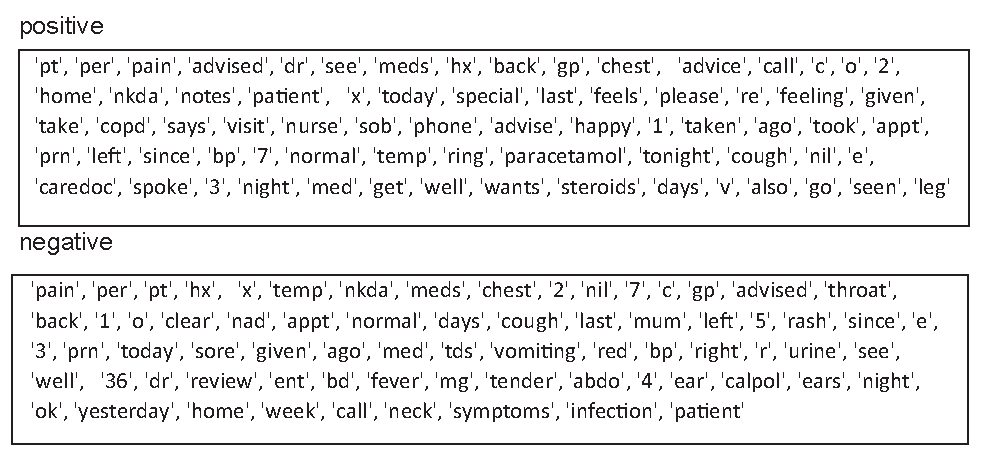
\includegraphics[scale=0.7]{word-frequency-nonpreprocessed.pdf}
       }
      \caption{Top seventy high occurring tokens in positive and negative cases respectively, excluding stopwords.}
      \label{word-frequency-nonpreprocessed}
   \end{figure}

%Looking at the top 
%
%    \begin{figure}[!ht]
%      \centering
%      \framebox{\parbox{2.5in}{
%}
%      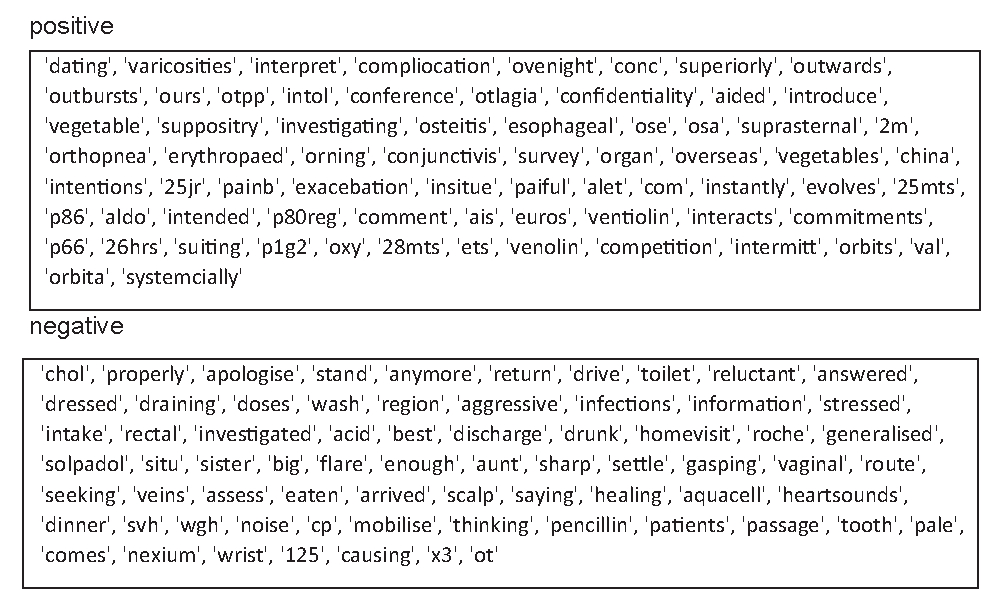
\includegraphics[scale=0.7]{word-tf-idf-unpreprocessed.pdf}
%       }
%      \caption{Top seventy tokens measured using TF-IDF}
%      \label{words-tf-idf-nonpreprocessed}
%   \end{figure}


%HOLD ON A SECOND! Naive Bayes\index{Naïve Bayes} USES TOP 100 WORDS? WELL THE TOP 70 WORDS FROM BOTH POSITIVE AND NEGATIVE CASES ARE VIRTUALLY IDENTICAL - SO WHAT... WHAT COULD IT POSSIBLY BE USING TO DERIVE AN ACCURATE RESULT IN RELATION TO TRUE POSITIVES? Lower the number of top words to 10, then to 1, to see how it does. If It still does well it is clearly cheating. Report most significant features.




%There's significant divergence between the TF-IDF tokens for positive and negative cases, as shown in Figure \ref{words-tf-idf-nonpreprocessed}. This would appear to augur well for predicting these cases. However, there are nevertheless significant issues with the highly ranked lexemes; perhaps somewhat intuitively indicated by the fact that clearly misspelled words (like `compliocation' or `pencillin') have ranked so highly. The OOHC\index{Out-of-hours Health Care} context of the data collection makes TF-IDF as a measure a little more problematic as repetition within case FTN is specifically avoided due to both temporal and comprehension considerations, while important measures may be relatively routine, thereby undercutting their apparent importance within the corpus as a whole. TF-IDF failed to produce any useful results with the classifiers, consequently the table below will relate results using most frequent terms, excluding stop-words.    




\subsubsection{Predictive performance}



 
 
 \begin{table}[h]
 \begin{center}

    \ra{1.4}
   \caption{Classification using bag-of-word\index{Bag-of-words representation} model.}
\begin{tabular}{|l|c|c|c|c|}
\hline
            & \textbf{Naive Bayes\index{Naïve Bayes}} & \textbf{SVM} & \textbf{RF} \\ \hline
Accuracy    & 0.26 $\pm 0.51$                & 0.66 $\pm 0.385$     & 0.68 $\pm 0.045$        \\ \hline
PPV         & 0.89 $\pm 0.53$               & 0.52  $\pm 0.459$    & 0.37 $\pm 0.015$            \\ \hline
NPV         & 0.24 $\pm 0.019$               & 0.49 $\pm 0.412$     & 0.69 $\pm 0.044$           \\ \hline
TPR         & 0.013 $\pm 0.001$               & 0.01 $\pm 0.0049$     & 0.006 $\pm 0.001$           \\ \hline
\end{tabular}
\label{table:ml-classification-bow}
 \end{center}
\end{table}

The results for the BOW model using the top 100 words can be seen in Table \ref{table:ml-classification-bow}. The average depth of the RF was 31.5. Naive Bayes\index{Naïve Bayes} in this instance was strongest at detecting true positives, while the RF algorithm was strongest at detecting true negatives (and consequently exhibited the best accuracy of the three algorithms tested).  

Owing to Naive Bayes\index{Naïve Bayes}' high PPV when using BOW\index{Bag-of-words representation} data, and high NPV when using parameterised data, experimentation combining both sets of data were used with this algorithm, in the event that some sort of equilibrium between true positive and true negative prediction could be attained. However, this combination merely furthered the algorithm's bias towards true negatives, with an average PPV score of 0.25 $\pm 0.47$ , and average NPV score of 0.89 $\pm 0.23$  when using this hybridised dataset.


\subsection{Summary}
\label{C}

Attempts to classify cases using more traditional machine learning techniques provided, at best, what could be described as modest results. While the lion's share of valuable information in relation to cases resided within FTN, performance of the algorithms using free text was not significantly superior to results borne from parameterised data. These results provided useful baselines from which to work, and indicated that classification using either textual data or paramaterised data would be theoretically possible. What these results did not provide was any indication the extent to which context could play a role in the use of FTN data. Although variants of the machine learning approaches taken above could theoretically provide improved performance (e.g. multinomial Naïve Bayes \cite{meftouh2019smart} or kernal based SVM), ultimately the decision was taken to focus on attempting to classify patients using FTN data by applying an artificial neural network model.



\section{Artificial Neural Networks}
\label{section:ANN-(theory)}
%\subsection{Motivation} 
When approaching the use of FTN; while the most important lexemes present in the corpus could hypothetically be extracted from cases for any classification purpose, such a position raises the question of how one would define what was, and was not, a significant lexeme in the first place. 

Intuitively, medical terms would seem to possess more importance in classifying cases. After all, physicians base their entire professions around the use of signs, symptoms, and histories of prescriptions and morbidities in their assessment of cases (though it should be noted that it would be virtually unheard of for doctors to actually provide a diagnosis based solely on textual information). Notwithstanding the conceptual soundness of this idea, the actual quality of the notes put paid to notions of using NER to this end. Typographical errors, widespread use of contractions, and a plurality of forms that different entities could take made the idea of using a predefined list of terms fundamentally unsound as a means of extracting useful features (at least in isolation).

A more general point is that this difficulty is present even if one presupposes that one's intuition concerning a certain type of word is correct. By this, it means that while it is reasonable to assume that the occurrence of symptoms and diseases in the text are significant (because they would in the context of diagnostics performed by humans), this does not necessarily mean that these particular terms (if one could even find them) are the only, or even the most important features present to solve the thesis problem. As has already been established in Section \ref{section:frequent-users-rr}, there is no accepted set of characteristics to define frequent users. As such, feature selection based upon human reasoning is, in this context, rendered somewhat moot. 

The last point ties into the choice of Artificial Neural Networks (ANNs\index{Artificial Neural Networks}) for the purposes of FTN classification. ANNs\index{Artificial Neural Networks} have in recent years been increasingly applied in natural language contexts and specifically, have had proven applicability in relation to data that has traditionally proven problematic in probability analytics and machine learning \cite{goldberg2017neural}. A particular consideration is the present context, whereby the chosen machine learning application must itself be able to learn from a sparse dataset what features represent strong information gain. Because of both the high volume of features (that is to say, unique words) and relatively high volume of data available to train models, ANNs\index{Artificial Neural Networks} presented a logical step in attempting to classify frequent user cases using FTN. 


The actual choice of neural network architecture was non-obvious. So too was the choice of data representation. Consequently an exhaustive series of tests were conducted to find to most suitable combination. It was also initially uncertain whether FTN alone or some combination with parameterised data would be prove optimal. However, before considering the methodology adopted to try and develop a solution, let us first look at what is meant by both Neural Networks in general, and specifically how recent research has appropriated them for FTN classification.  

Artificial Neural Networks are loosely modelled on their biological equivalent, and are constructed as a collection of neurons (or perceptrons) \cite{rosenblatt1957perceptron} organised in a sequence of one or more hidden layers \cite{goldberg2017neural}. Typically these networks are multiple layers deep (hence the relatively redundant term of `deep learning') where neurons receive as input the neuron activations from the previous layer \cite{rumelhart1988learning}. Neuron activations perform a weighted sum of the input typically followed by a non-linear activation function. While weights are essentially composed of random values to begin with (though the manner in which these values are generated differs depending on initialisation method used) \cite{steinwart2019sober}, backpropagation is typically a method used to adjust the connection weights to minimise the error during learning \cite{rumelhart1988learning}. 

Activation functions to find non linear error gradients can thus be used in tandem with backpropagation to find complex patterns in data. The updating of weight values is performed by an optimisation algorithm \cite{goodfellow2016deep}. However, there are multiple different activation functions and optimisation algorithms that one may use to this effect. While different activation functions and optimisation algorithms have different strengths and weaknesses, it is hard to justify an \textit{a priori} choice with relation to these components \cite{wolpert1997no}. 

Multi-Layer Perceptrons (MLP\index{Multi-Layer Perceptrons}) are neural networks with more than one layer while Convolutional Neural Networks (CNN\index{Convolutional Neural Networks}) are, simply put, neural networks that use convolution in place of general matrix multiplication in at least one of their layers. Convolution is defined as follows

\begin{equation}
s(t) = (x*w)t = \sum_{i=-\infty }^{\infty} x(i)w(t-i) 
\end{equation}

\textit{W}here \textit{x} is a vector of inputs, \textit{w} is a vector of weights, \textit{i} is an index variable, and \textit{t} is time (or window) \cite{goodfellow2016deep}.

CNNs may have pooling layers to perform non-linear downsampling. CNNs are exceptionally popular in vision recognition tasks, but as will become apparent, have had significant recent application in FTN contexts. 









Recurrent Neural Networks (RNN\index{Recurrent Neural Network}) are different from both MLP and CNN in that MLP and CNN are both feed-forward networks, in the sense that the connections
between neurons do not form cycles or loops. Feedforward networks make an assumption of independence between inputs, whereas Recurrent Neural Networks, as the name may suggest, have a looping mechanic, in the form of at least one feedback connection \cite{rumelhart1988learning}. This allows this type of architecture to treat the interdependence of sequential data. A consequence of this is that while CNNs may be able to consider the immediate context of input (for instance a local group of pixels or characters), they cannot understand temporal connections. A major limiting factor for RNN\index{Recurrent Neural Network} is that traditional, fully connected RNN\index{Recurrent Neural Network} tend to suffer from both vanishing and exploding gradients as weights are backpropagated through the recursive layers (where the model may forget earlier input, or be subject to instability) \cite{goodfellow2016deep}. The most common method to solve this deficiency is the use of a gating mechanic. 











 \section{Approaches}
\label{section:ann-approaches}

%Multi-Layer perceptrons do not take context into account

%Convolutional Neural Networks (CNNs) mix together partial information gathered from what it's looking at. 

%Recurrent Neural Networks repeat

%Gating can be used to



The use of machine learning in relation to medical data is by no means new. However, free-text\index{free-text} has proven a problematic source of features for classic machine learning techniques. Even when advanced feature extraction methodologies are employed, the inherent noise and heterogeneity of medical natural language remains an issue. Current research within medical informatics have begun to broach ANNs\index{Artificial Neural Networks} for use with data from Electronic Health Records in order to overcome these challenges. 

Issues can arise when establishing ground truth in analysis. If training data has to be generated manually by domain experts, this often results in relatively small datasets, which typically provides a poor basis upon which to use deep learning methodologies \cite{gehrmann2018comparing,geraci2017applying,yao2016convolutional}.  While this thesis can avoid this issue, particular to hand-curated datasets, as discussed in Section \ref{section-rr-medical-text}, there nevertheless is a ceiling on the volume of data that can be used in training a neural network model, owing to the fact that the classification system being developed specifically concerns outlier cases. 

However, the actual use of neural networks in conjunction with EHR\index{Electronic Health Record} has displayed wide variance in contemporary research. For instance, some researchers maintain feature extraction techniques, and use neural networks for classification purposes using these extracted features, while others use neural networks for the purposes of feature transformation, and have other types of machine learning algorithms use these features. The architectures and designs of the ANNs\index{Artificial Neural Networks} similarly are multivariate, with no single structure proving the de facto standard across extant research.

Geraci et al. for instance use MLP\index{Multi-Layer Perceptrons} as part of H2O.ai's Deep Learning platform \cite{geraci2017applying}. Similar to the objectives of this thesis, Geraci et al. seek to produce a binary classification of patients, in their case, as either suitable or unsuitable to be participants for a study on youth depression. The data Geraci et al. were considering was unstructured medical textual notes with limited application of diagnosis codes. 

Geraci et al. accepted that searching using a fixed list of terms could potentially achieve a reasonably high accuracy \textit{vis-à-vis} the correct identification (or exclusion) of potential candidates. Contextual negation was also taken into account for list based searches. On very select training sets this ``brute-force" methodology could obtain 80\% sensitivity and 88\% specificity. However, as these researchers expected, this approach did not generalise, and in some cases during cross validation it achieved no better than random accuracy.

Geraci et al. were faced with a relatively small dataset, as classification had to be performed by domain experts, leaving a total of 861 patient documents with which to work. The actual features of the documents were refined into a document term matrix, with the value for each term recorded by its TF-IDF ratio. Somewhat unusually, Geraci et al. produced two separate neural network models, one which had high specificity and poor sensitivity, and one which happened to have high sensitivity but poor specificity. By combining the results of these two neural networks Geraci et al.'s model achieved a sensitivity of 75\% and specificity of 87\%. The actual structure of the neural networks was that of a three layer network, with relu activation function on hidden layers. The significant difference between the high sensitivity and specification networks was the number of nodes, with the high specificity network having 758 input nodes, with the high sensitivity network having 102 input nodes. Other aspects relating to the architecture of either network are not looked at at length.

% Unlike Geraci et al., the dataset under investigation was substantial (comprising aggregated EHR\index{Electronic Health Record} data of some 700,000 patients, of which 76,214 were used for testing purposes).

The use of neural networks using unsupervised learning for the purposes of preprosessing of features is fairly typical in NLP applications. This is increasingly common for natural language in medical domains, as can be seen, for instance in Miotto et al.'s DeepPatient classifier project which uses a denoising autoencoder\cite{miotto2016deep}. Although DeepPatient ultimately uses a RF for the purposes of classifying patients,  the use of autoencoders clearly improved the quality of the medical textual features presented. DeepPatient's preprocessing saw dramatic improvements in detection of certain disorders, over that achieved using raw text, but this was not shared uniformly. Similarly the use of unsupervised ANNs\index{Artificial Neural Networks} to produce word embeddings, typically using Google's Word2Vec\index{Word2Vec}, has been employed to improve results of systems such as the named-entity recognition described by Habibi et al. \cite{habibi2017deep}. 

Rasmy et al. use the Reverse Time AttentIoN  (RETAIN) RNN\index{Recurrent Neural Network} model for the prediction of heart disease based on the extracted information from Electronic Health Records \cite{rasmy2018study}. While this objective is similar to this thesis' planned capacity to detect frequent users, Rasmya et al.'s data does not seem to include natural language. Importantly, Rasmy et al. demonstrated the generalisability of RNNs\index{Recurrent Neural Network}, given a corpora from different hospitals, and the superior performance of the RNN\index{Recurrent Neural Network} used in such classification compared to a more traditional model such as logistic regression.

In counterpoint, C. Yao et al. use a Convolutional Neural Network (CNN \index{Convolutional Neural Networks}) in order to predict correct answers to users' questions in an online Q\&A system \cite{yao2016convolutional}. The specific structure used in this CNN \index{Convolutional Neural Networks} is inherited from the work by Yoon Kim 
%[]
\cite{kim2014convolutional}. A large amount of preprocessing of textual data is performed on the user submitted data, with an emphasis on extracting symptoms, though these features are also vectorised as word embeddings. The accuracy of the model that C. Yoa et al. create is 71\%. It is shown in this research that the quality of the predictions in this case is largely dependent upon the number of symptoms that are present in user data. 

Gehrmann et al. also use Kim's CNN\index{Convolutional Neural Networks} architecture to attempt to identify particular patient phenotypes from patterns discovered in their medical notes \cite{gehrmann2018comparing}. In particular, as is the case in the research in this thesis, specific emphasis was placed on the identification of ``frequent flyer" patients; that is to say, patients that have an unusually high amount of contact with the healthcare facility in question. Due to the necessity of manual annotation, the dataset in Gehrmann et al.'s research was small, with some 1610 cases available for both training and testing purposes.    

Gehrmann et al. automatically extracted clinical features using cTAKES \cite{gehrmann2018comparing}, which were then used as the features in the CNN\index{Convolutional Neural Networks}. Like many of the other papers presented here, these features were provided to the classifier as a bag-of-words\index{Bag-of-words representation}. However, prior to their treatment by the CNN \index{Convolutional Neural Networks}, the words were transformed into word embeddings using Word2Vec. The CNN \index{Convolutional Neural Networks} achieved a high F-score across all tests, though results differed significantly, depending on the specific phenotype being tested. 


The use of unsupervised artificial neural networks\index{Artificial Neural Networks} to preprocess data is well established, and improvements seen in the quality of features derived from unstructured medical text is similar to that observed in other natural language domains \cite{miotto2016deep}. The use of some type of ontology to attempt to improve features is also sometimes seen \cite{gehrmann2018comparing}. The actual quality of unstructured medical text can vary wildly (both between different datasets and often within the same dataset). If individual cases are being classified, both the volume of data in individual cases, and the quality that this data is presented may form a limiting factor for the effectiveness of any classification algorithm \cite{yao2016convolutional} .

\begin{figure}[htbp]
   \begin{center}

 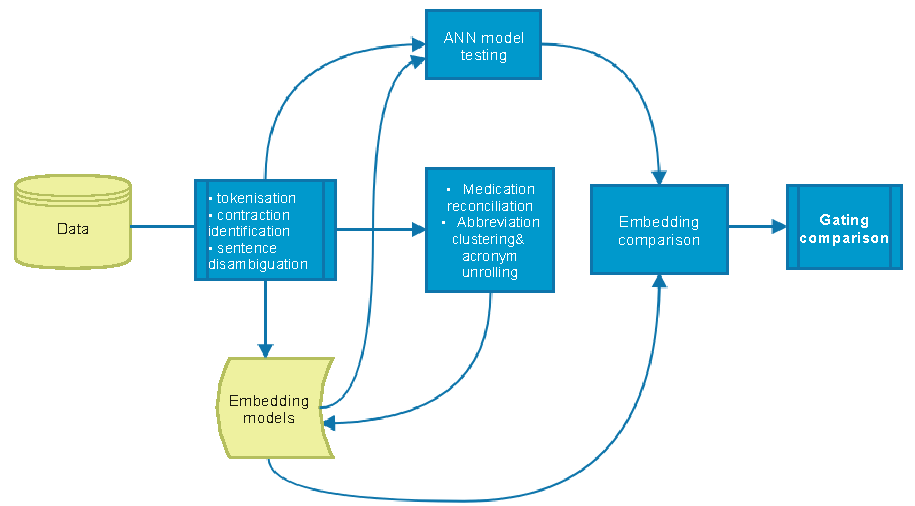
\includegraphics[width=1.0\textwidth]{Figs/scheme-development-plan-.pdf} 

 \caption{High level overview of system development.}
 \label{fig:development-plan}
  \end{center}
\end{figure}


%Similar to C. Yao et al's solution

All of the literature discussed above shows the potential strength of artificial neural networks\index{Artificial Neural Networks} in connection with EHR\index{Electronic Health Record}. However, while many of these papers compare artificial neural networks\index{Artificial Neural Networks} with other machine learning methodologies, less focus is placed on the specific type, parameters, or hyperparameters of the artificial neural network used within the scope of their analyses. 




%Cut and paste the related research from chapter 5 in here after the initial section on ANNs\index{Artificial Neural Networks} .... possibly Free-Text use of Deep Learning


A high level depiction of the methodology adapted in determining the optimal combination of neural network architecture and data representations can be seen in Figure \ref{fig:development-plan}. Note that this figure is created retrospectively (when it was already determined that a Neural Network with gating mechanic would be most ideally suited to the problem). \hl{The preprocessing steps were not entirely linear, as some processes were mutually dependent. For instance, contraction identification was necessary for effective sentence disambiguation, and sentence disambiguation was necessary for training of word embedding models. To elaborate on this point, distinguishing between full stops that formed part of contractions, and those that indicated the ends of sentences was integral to the development of training data for the generation of word embeddings.  However, the word embedding model was necessary for finding many of the long forms of abbreviations used within the corpus. The act of preprocessing itself necessitated the retraining of word embeddings to cope with the altered textual data within the corpus.} Figure \ref{fig:development-plan} also depicts the testing of the competing models of ANN\index{Artificial Neural Networks} initially considered, namely Multilayer Perceptrons, Convolutional Neural Networks, and the use of gating in the context of Recurrent Neural Networks. 








%Results in the literature suggest that artificial neural networks, particularly those which feature deep neural layers, have strong predictive power and generalize well in relation to unstructured textual data.

%\subsection{Aim}






\section{Summary}


This chapter has established the non-trivial task of attempting to classify frequent users. Although different ML approaches to classifying patient cases had diverse results, it would be hard to declare any particular algorithm as obviously superior. Nonetheless it is clear that features present in the dataset can be used to classify patients. Given the challenging nature of the data, artificial neural networks\index{Artificial Neural Networks} appear to be good alternative to more traditional ML approaches. However, the network most appropriate to the task at hand is initially unclear. Existing research into use of FTN has not displayed any single network type as indisputably superior. Furthermore, given that the specific dataset under investigation in the course of this thesis has not been subject to any prior ML research, evaluation of different methods of data representation would appear warranted.     


